%!TEX program = xelatex
%%%%%%%%%%%%%%%%%%%%%%%这是导言部分的开始%%%%%%%%

%========= 导言部分声明文档的类型=================
\documentclass{article}

%=========导言部分可可以加载宏包=================
\usepackage{amsmath}                % 数学公式排版宏包
\usepackage{amssymb}                % 数学符号命令宏包
\usepackage{amsthm}                 % 数学定理宏包
\usepackage[UTF8]{ctex}             % 中文输入宏包
\usepackage[a4paper]{geometry}      % 页面设置宏包
\usepackage{setspace}               % 行间距宏包
\usepackage{graphicx}               % 图片宏包
\usepackage{listings}               % 代码宏包
\usepackage{color}					% 颜色宏包
\usepackage{xcolor}                 % 颜色处理宏包
\usepackage{float}                  % 浮动对象式样宏包
\usepackage{fontspec}
\usepackage{enumerate}				% 列举编号包

%=========页面设置==============================
\geometry{left=1cm,right=1cm,top=1cm,bottom=2cm}
\onehalfspacing
\setlength\parindent{0em}

%=========代码格式设置============================
\definecolor{dkgreen}{rgb}{0,0.6,0}
\definecolor{gray}{rgb}{0.5,0.5,0.5}
\definecolor{mauve}{rgb}{0.58,0,0.82}
% \setmonofont{Consolas}
\lstset{
	numbers = left, 	
	numberstyle = \color{gray}, 
	keywordstyle = \color{blue},
	commentstyle = \color{dkgreen}, 
	stringstyle = \color{mauve},
	basicstyle = \ttfamily,
	breaklines = true,
	frame = shadowbox, % 阴影效果
	rulesepcolor = \color{ red!20!green!20!blue!20} ,
	escapeinside = ``, % 英文分号中可写入中文
	xleftmargin = 2em,xrightmargin=2em, aboveskip=1em,
	framexleftmargin = 2em
} 

%=========导言部分可以定义标题信息===============
\title{组会报告}
\author{徐益}
\date{\today}
%%%%%%%%%%%%%%%%%%%%%%%这是导言部分的结束%%%%%%%%%

%%%%%%%%%%%%%%%%%%%%%%%这是正文部分的开始%%%%%%%%%
\begin{document}

%=========生成标题================================
\maketitle

%=========开始正文的输入==========================

%===========第一节=================
\section{工作内容}
1. 处理线程死锁Bug;

2. 更换线程绑定CPU方案;

3. 测试系统性能;

4. 修改开题报告。

%===========第二节=================
\section{更换线程绑定CPU方案}
\begin{figure}[H]
	\centering
	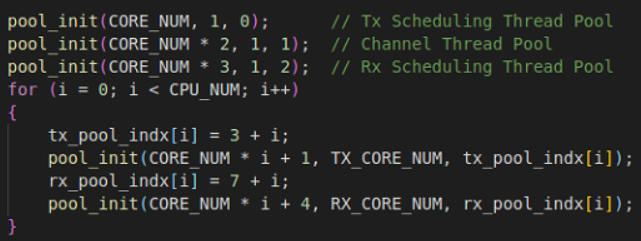
\includegraphics[width = .6\textwidth]{pool.png}
	\caption{新的线程绑定CPU方案}
\end{figure}
\begin{figure}[H]
	\centering
	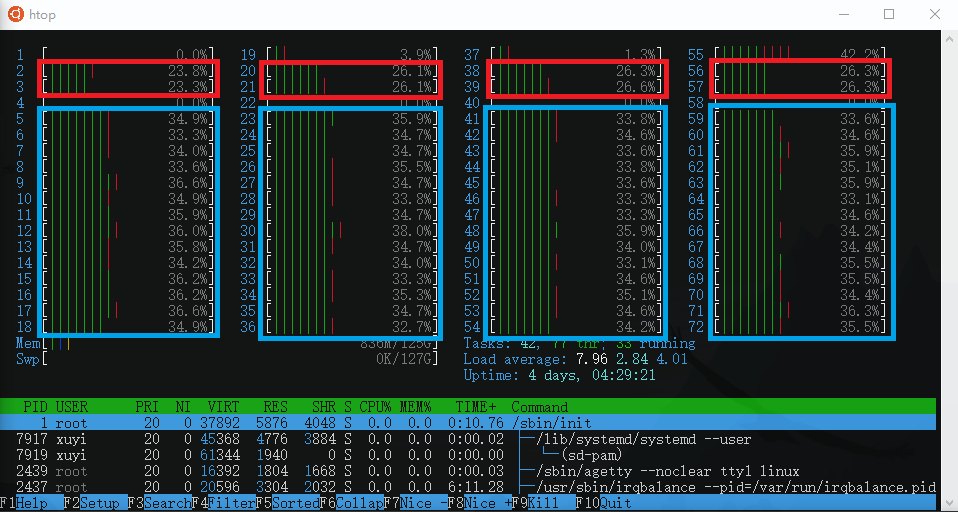
\includegraphics[width = .8\textwidth]{htop.png}
	\caption{CPU占用情况}
\end{figure}

%===========第三节=================
\section{测试系统性能}
\section{测试结果}
\begin{figure}[H]
	\centering
	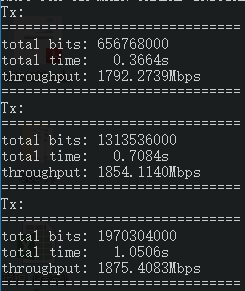
\includegraphics[width = .4\textwidth]{tx42.png}
	\caption{发送端性能}
\end{figure}
\begin{figure}[H]
	\centering
	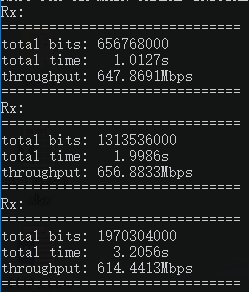
\includegraphics[width = .4\textwidth]{rx414.png}
	\caption{接收端性能}
\end{figure}
\section{CPU使用情况与吞吐量的关系}
\begin{table}[H]
	\caption{发送端CPU使用情况与吞吐量的关系}
	\centering
	\begin{tabular}{|l|l|l|l|l|l|l|}% 通过添加 | 来表示是否需要绘制竖线
		\hline  % 在表格最上方绘制横线
		CPU		& CORE		& Throughput	& Degree of Parallelism	\\
		\hline
		1		& 1			& 302.28Mbps	& 100.00\%				\\
		\hline
		4		& 1			& 1038.59Mbps	& 85.90\%				\\
		\hline
		4		& 2			& 1792.27Mbps	& 74.11\%				\\
		\hline  % 在表格最下方绘制横线
	\end{tabular}
\end{table}
\begin{table}[H]
	\caption{接收端CPU使用情况与吞吐量的关系}
	\centering
	\begin{tabular}{|l|l|l|l|l|l|l|}% 通过添加 | 来表示是否需要绘制竖线
		\hline  % 在表格最上方绘制横线
		CPU		& CORE		& Throughput	& Degree of Parallelism	\\
		\hline
		1		& 1			& 47.38Mbps		& 100.00\%				\\
		\hline
		4		& 1			& 176.62Mbps	& 93.19\%				\\
		\hline
		4		& 2			& 298.13Mbps	& 78.65\%				\\
		\hline
		4		& 3			& 388.55Mbps	& 68.34\%				\\
		\hline
		4		& 4			& 418.02Mbps	& 55.41\%				\\
		\hline
		4		& 5			& 512.31Mbps	& 54.06\%				\\
		\hline
		4		& 6			& 521.66Mbps	& 45.88\%				\\
		\hline
		4		& 7			& 520.70Mbps	& 39.25\%				\\
		\hline
		4		& 8			& 610.47Mbps	& 40.26\%				\\
		\hline
		4		& 9			& 615.41Mbps	& 36.08\%				\\
		\hline
		4		& 10		& 604.59Mbps	& 31.90\%				\\
		\hline
		4		& 11		& 609.78Mbps	& 29.25\%				\\
		\hline
		4		& 12		& 609.33Mbps	& 26.79\%				\\
		\hline
		4		& 13		& 586.91Mbps	& 23.82\%				\\
		\hline
		4		& 14		& 674.87Mbps	& 25.44\%				\\
		\hline  % 在表格最下方绘制横线
	\end{tabular}
\end{table}
\subsection{其他问题}
\begin{figure}[H]
	\centering
	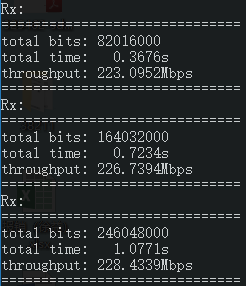
\includegraphics[width = .4\textwidth]{rxs42.png}
	\caption{单流4CPU2CORE}
\end{figure}
\begin{figure}[H]
	\centering
	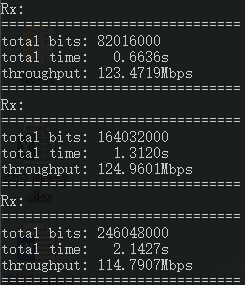
\includegraphics[width = .4\textwidth]{rxs414.png}
	\caption{单流4CPU14CORE}
\end{figure}

%===========第四节=================
\section{已做过的尝试和待实现的尝试}
\subsection{已做过的尝试}
1. 在按线程池分配CPU后,再修改线程亲和度。(性能未提升)

2. 在发送端改为轮询调度结构。(性能未提升)

\subsection{待实现的尝试}
1. 按CPU分配运算空间。

2. 修改线程池源码。

%===========第五节=================
\section{修改开题报告}


%===========下周计划=================
% \section{下阶段计划}
% 1. 尝试解决上述问题;

% 2. 准备开题。

\end{document}
%%%%%%%%%%%%%%%%%%%%%%%这是正文部分的结束%%%%%%%%%%%%